\documentclass[]{article}
\usepackage{amsmath}
\usepackage{amsthm}
\usepackage{listings}
\usepackage{graphicx}
\usepackage{hyperref}
%\usepackage{cleveref} %for the cref command

\title{Practical Lab Numerical Computing Computational Finance \\Bachelor-Worksheet 3}
\author{Lukas Troska, Ilja Kalmykov}
\date{}
\setlength{\parindent}{0pt}

\begin{document}

\maketitle

The referenced source code files can be found on
\url{https://github.com/iljaGH/CompFin/}.

\section*{Task 2}
See task2.cpp for code.

\section*{Task 3}
As we can see, the number of time steps does not
affect the convergence at all.
\begin{figure}[!ht]
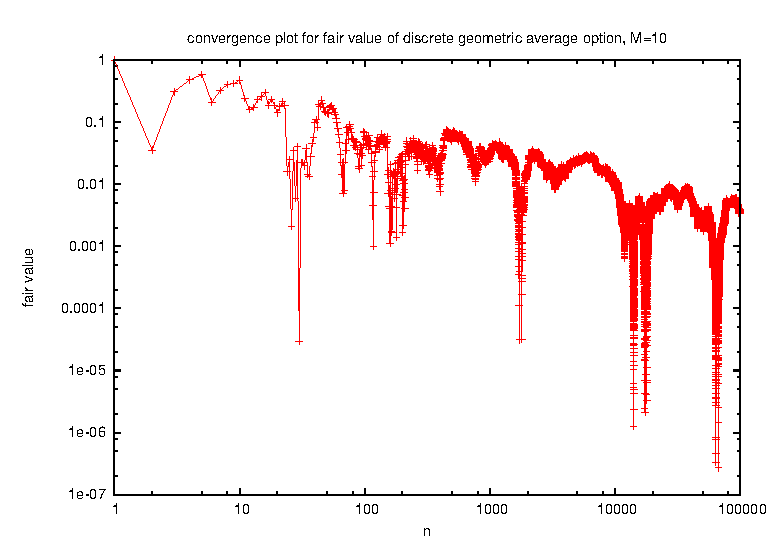
\includegraphics[width=.9\textwidth]{task3_10.eps}
\caption{Convergence plot for the fair value of diskrete geometric average
option, $M = 10$.}
\label{fig:Task3a}
\end{figure}
\begin{figure}[!ht]
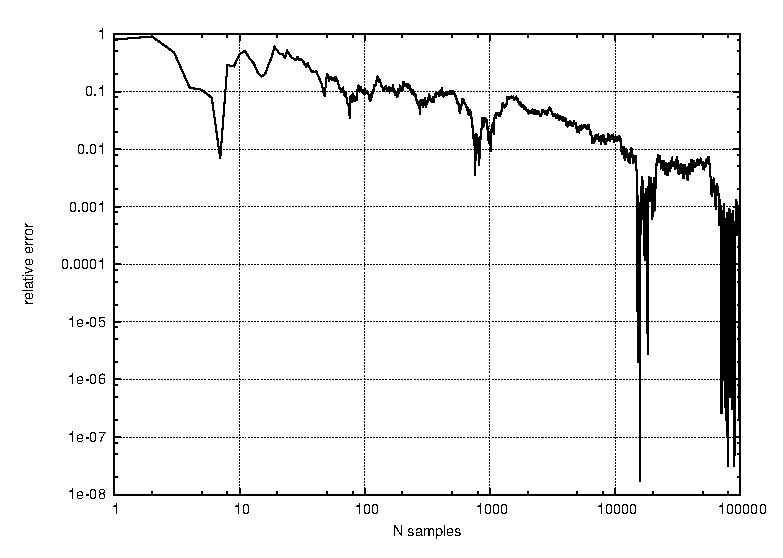
\includegraphics[width=.9\textwidth]{task3_200.eps}
\caption{Convergence plot for the fair value of diskrete geometric average
option, $M = 200$.}
\label{fig:Task3b}
\end{figure}
\clearpage

\section*{Task 4} See task4.cpp for code. The convergence
is $N$. The last increase in error is because of the limitations of
the datatype int. For $M\ge 1024$ we get under-/overflows in our calculation
because the numbers are too big.
\begin{figure}[!ht]
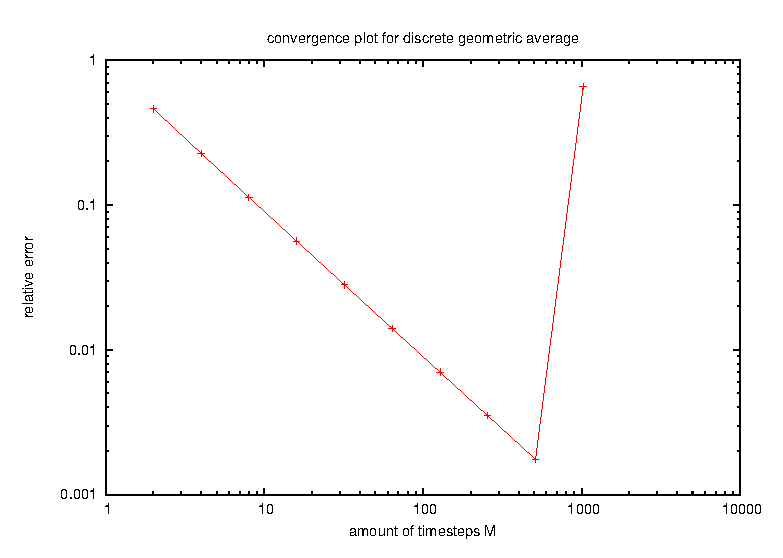
\includegraphics[width=.9\textwidth]{task4.eps}
\caption{Convergence plot for the diskrete geometric average.}
\label{fig:Task4}
\end{figure}
\clearpage

\section*{Task 5} See task5.cpp for code. The
integrand of the discrete arithmetic average for $M=2$ looks like:\\
\begin{figure}[!ht]
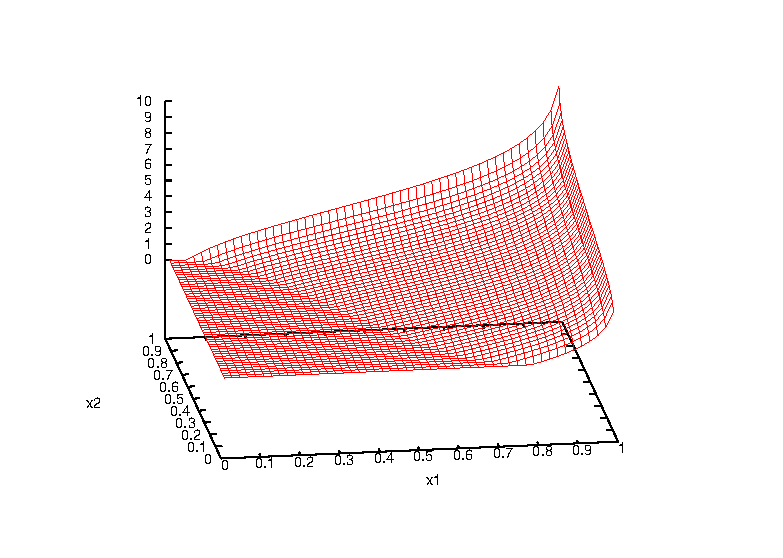
\includegraphics[width=.9\textwidth]{task5_1}
\caption{Integrand of discrete arithmetic average, $M=2,S(0)=10,r=0.1,\sigma=0.25,T=1,K=10$}
\label{fig:Task5}
\end{figure}
\clearpage

\section*{Task 6}
See task6.cpp for code.

\section*{Task 7} See task7.cpp for code. The first plot is a plot of the
first 100 members of the Halton sequence for $d=2$ and 100 uniform random numbers on
$(0,1)^2$ in the second plot. As we can see, the Halton sequence covers the
unit square more evenly than uniformly distributed points, i.e. "gaps" between the points are not as
big.\\
\begin{figure}[!ht]
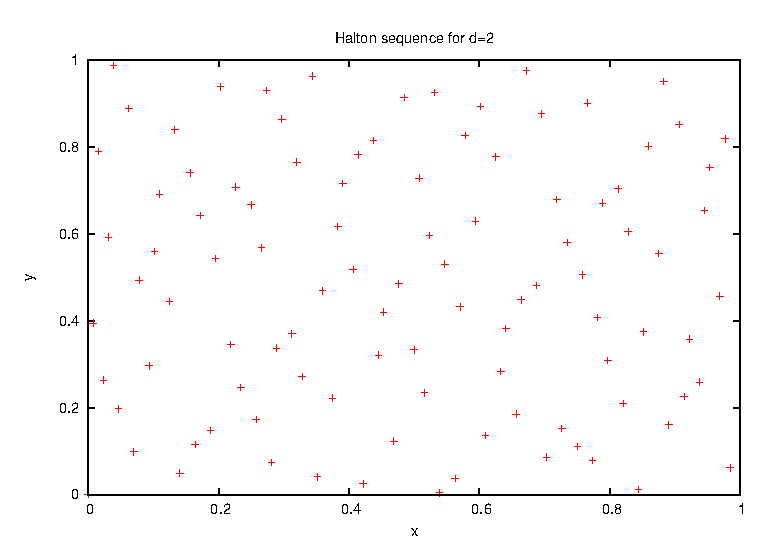
\includegraphics[width=.9\textwidth]{task7_halton.eps}
\caption{Halton sequence (2-dimensional, first 100 members)}
\label{fig:Task7a}
\end{figure}
\begin{figure}[!ht]
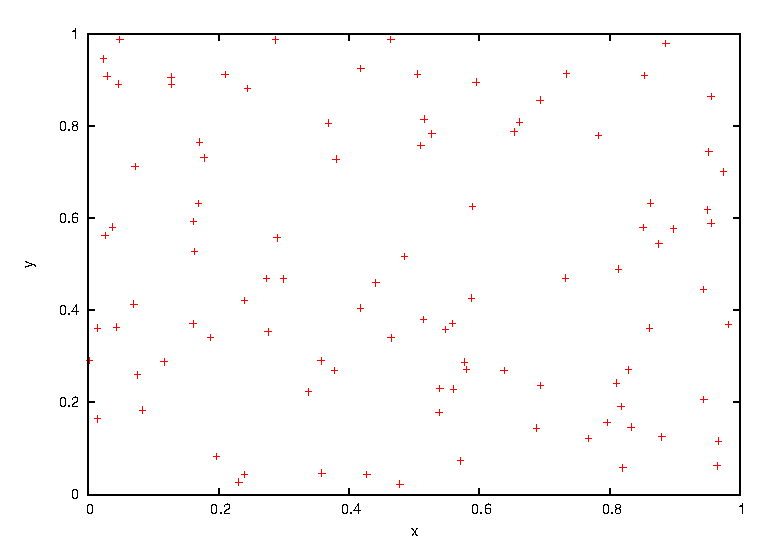
\includegraphics[width=.9\textwidth]{task7_uniform.eps}
\caption{100 uniform random numbers on $(0,1)^2$}
\label{fig:Task7b}
\end{figure}
\clearpage




\section*{Task 8}
See task8.cpp for code.

\section*{Task 9}
\begin{figure}[!ht]
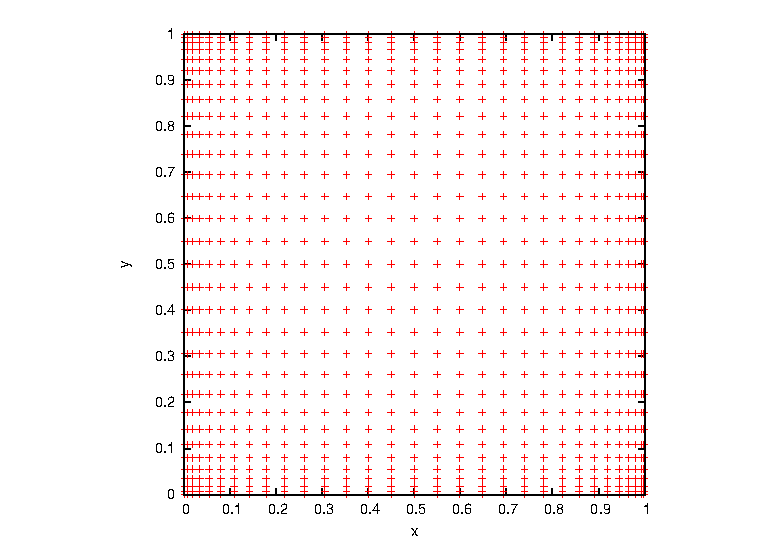
\includegraphics[width=.9\textwidth]{task9_gauss}
\caption{product rule grid for Gauss-Legendre at level 5}
\label{fig:Task9a}
\end{figure}

\begin{figure}[!ht]
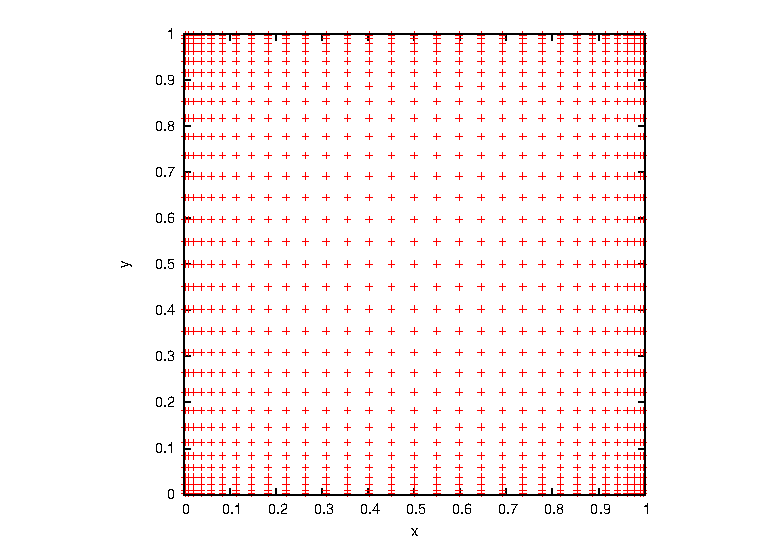
\includegraphics[width=.9\textwidth]{task9_cc}
\caption{product rule grid for Clenshaw-Curtis at level 5}
\label{fig:Task9b}
\end{figure}

\begin{figure}[!ht]
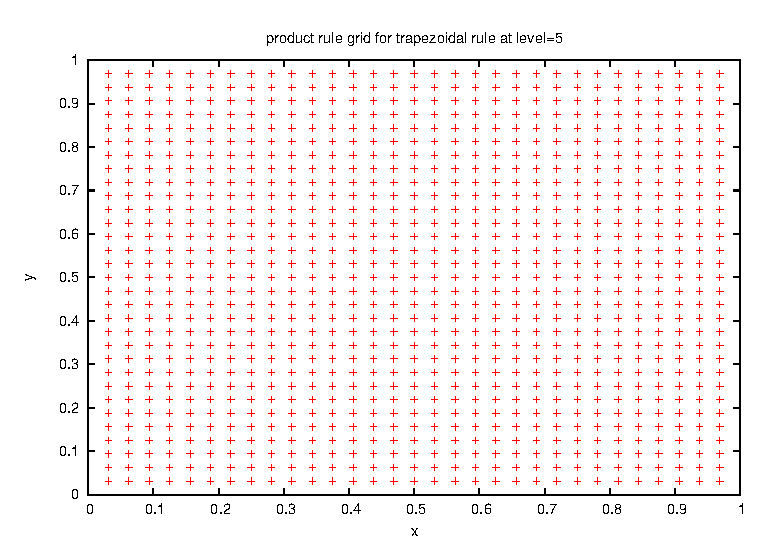
\includegraphics[width=.9\textwidth]{task9_trapezoidal}
\caption{product rule grid for trapezoidal rule at level 5}
\label{fig:Task9c}
\end{figure}
\clearpage





\section*{Task 10}
See task10.cpp for code.

\section*{Task 11}
\begin{figure}[!ht]
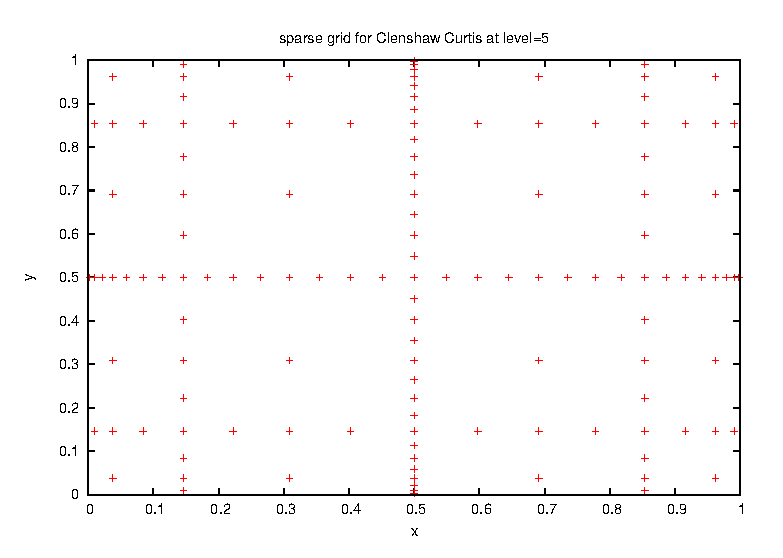
\includegraphics[width=.9\textwidth]{task11_cc5}
\caption{sparse grid for Clenshaw-Curtis at level 5}
\label{fig:Task11a}
\end{figure}

\begin{figure}[!ht]
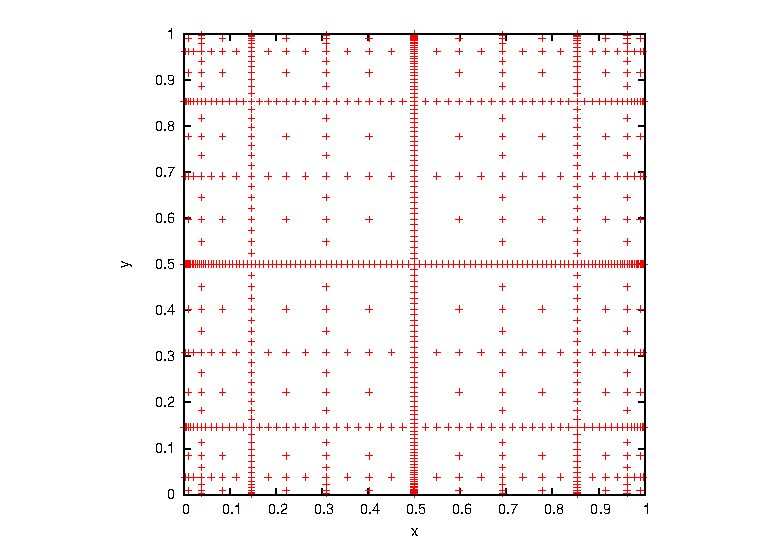
\includegraphics[width=.9\textwidth]{task11_cc7}
\caption{sparse grid for Clenshaw-Curtis at level 7}
\label{fig:Task11b}
\end{figure}

\begin{figure}[!ht]
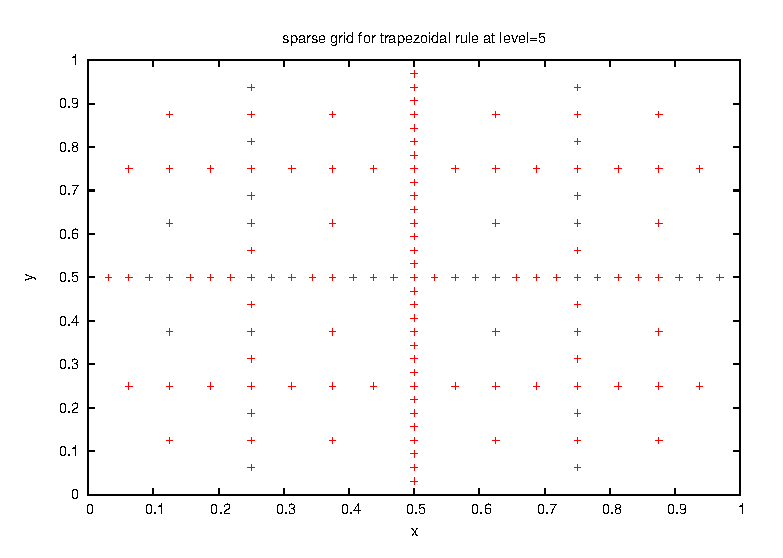
\includegraphics[width=.9\textwidth]{task11_trap_5}
\caption{sparse grid for trapezoidal rule at level 5}
\label{fig:Task11c}
\end{figure}

\begin{figure}[!ht]
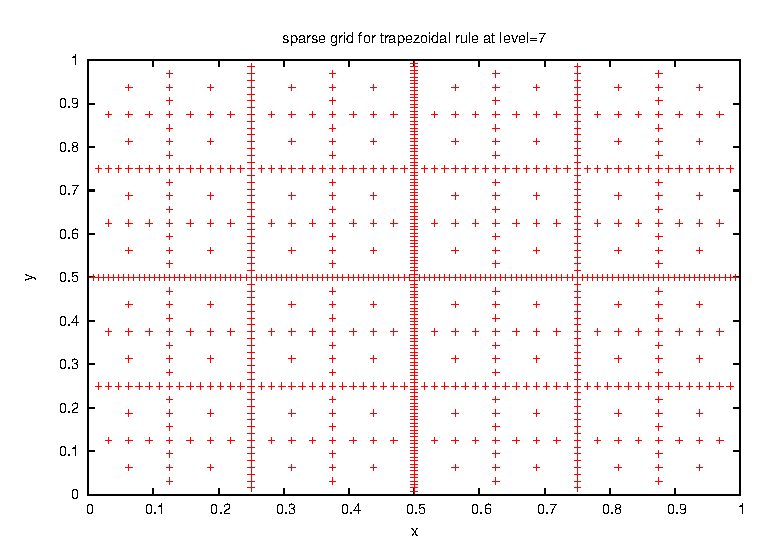
\includegraphics[width=.9\textwidth]{task11_trap_7}
\caption{sparse grid for trapezoidal rule at level 7}
\label{fig:Task11d}
\end{figure}
\clearpage





\section*{Task 12}
\begin{figure}[!ht]
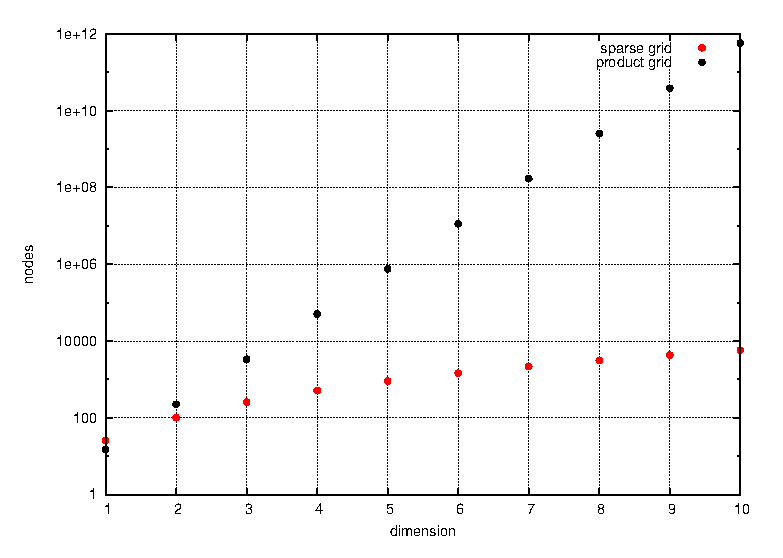
\includegraphics[width=.9\textwidth]{task12}
\caption{number of points/evaluations for sparse grid/product grid of level 4}
\label{fig:Task12}
\end{figure}


\section*{Task 13}
Convergence plots for integrating $f(x_1,...,x_d)=\prod_{j=1}^d (1+\gamma*\exp(x_j/2)),\gamma=0.1$.\\
\begin{figure}[!ht]
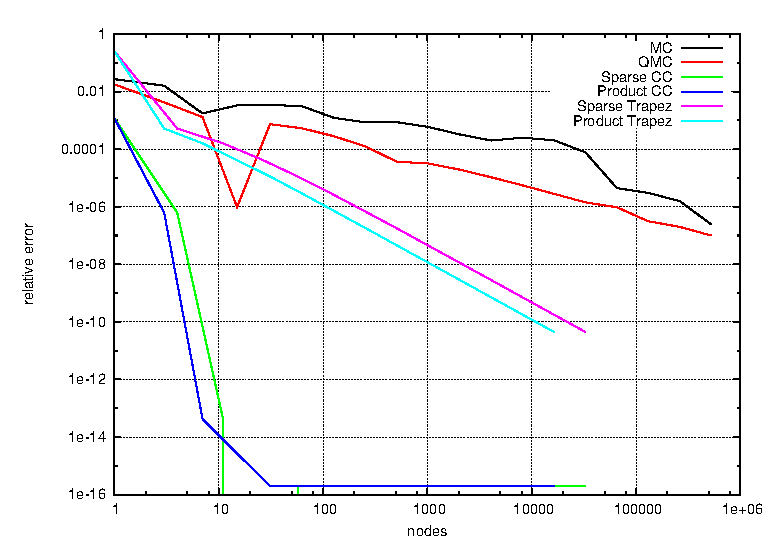
\includegraphics[width=.9\textwidth]{task13_d1}
\caption{convergence plot for $d=1$}
\label{fig:Task13a}
\end{figure}

\begin{figure}[!ht]
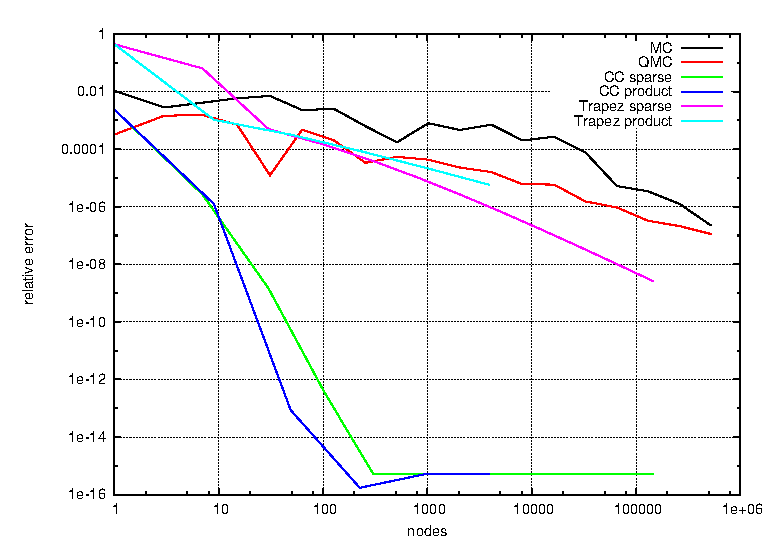
\includegraphics[width=.9\textwidth]{task13_d2}
\caption{convergence plot for $d=2$}
\label{fig:Task13b}
\end{figure}

\begin{figure}[!ht]
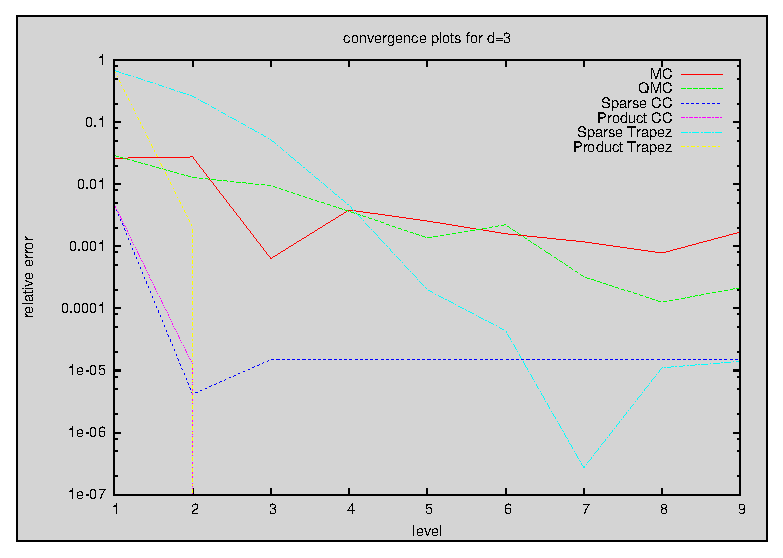
\includegraphics[width=.9\textwidth]{task13_d4}
\caption{convergence plot for $d=4$}
\label{fig:Task13c}
\end{figure}

\begin{figure}[!ht]
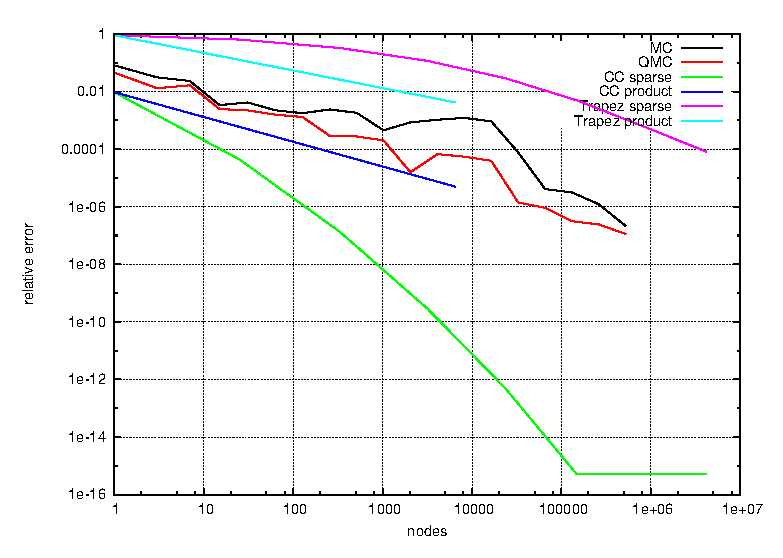
\includegraphics[width=.9\textwidth]{task13_d8}
\caption{convergence plot for $d=8$}
\label{fig:Task13d}
\end{figure}
\clearpage

\section*{Task 14}
See task14.cpp/task15.cpp

\section*{Task 15}
\begin{figure}[!ht]
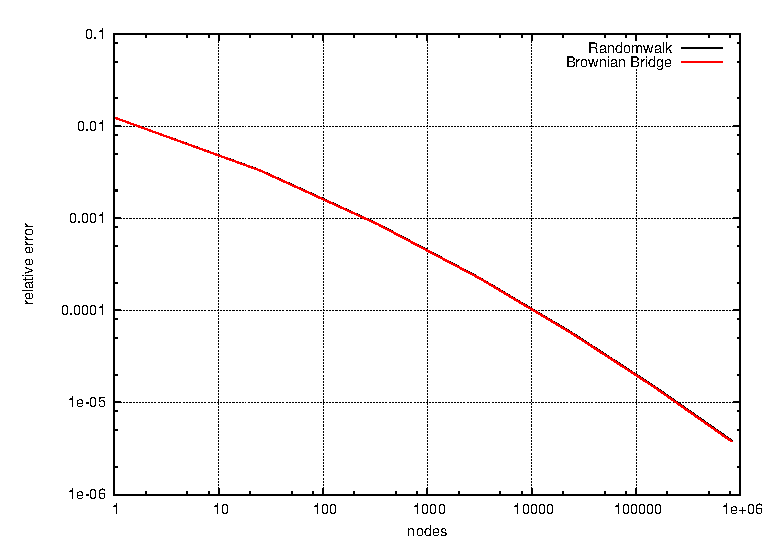
\includegraphics{task15}
\caption{convergence plot for Clenshaw-Curtis sparse grid for randomwalk/Brownian Bridge on discrete geometric Asian option, $S(0)=10,r=0.1,\sigma=0.25,T=1,M=16,K=0$}
\label{fig:Task15}
\end{figure}
\clearpage

\section*{Task 16}
Integration of discrete geometric Asian optien with parameters $S(10)=10,r=0.1,\sigma=0.25,T=1,K=0,M=8$.

\begin{figure}[!ht]
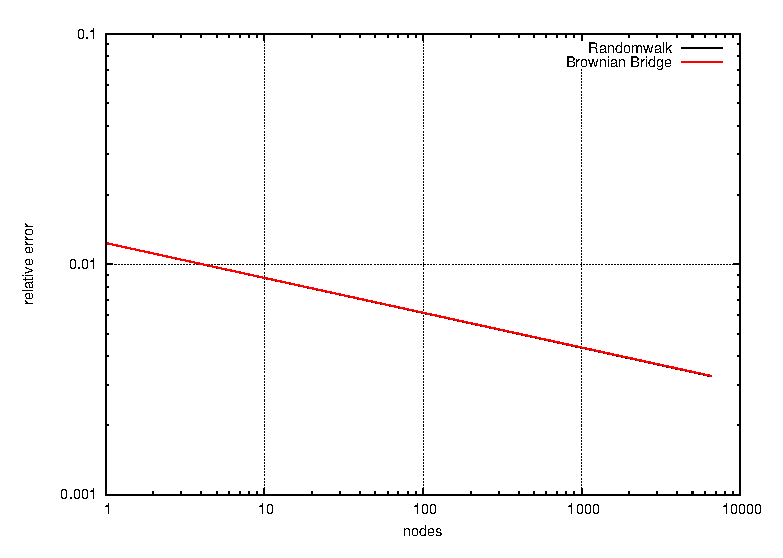
\includegraphics{task16_ccprod}
\caption{Product grid Clenshaw-Curits}
\label{fig:Task16a}
\end{figure}

\begin{figure}[!ht]
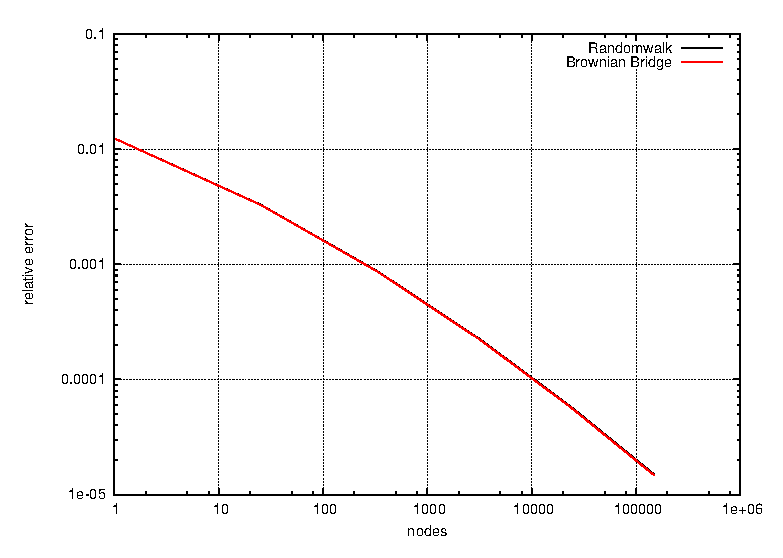
\includegraphics{task16_ccsparse}
\caption{Sparse grid Clenshaw-Curtis}
\label{fig:Task16b}
\end{figure}

\begin{figure}[!ht]
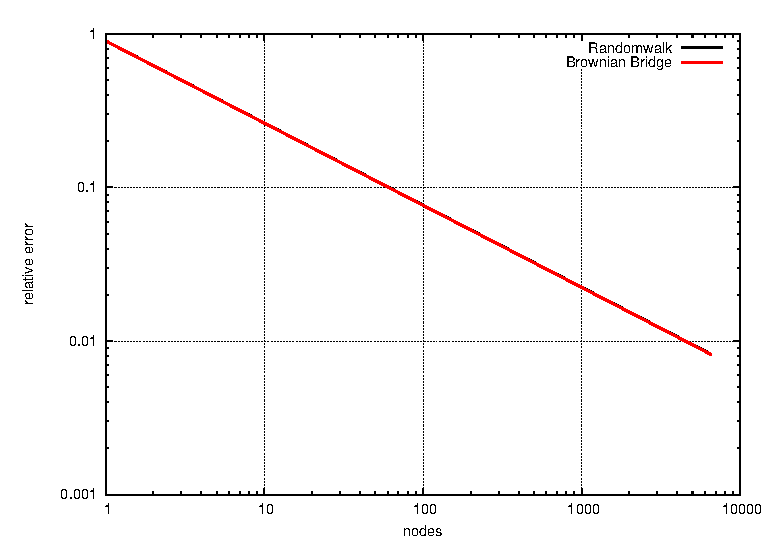
\includegraphics{task16_trapprod}
\caption{Product grid trapezoidal rule}
\label{fig:Task16c}
\end{figure}

\begin{figure}[!ht]
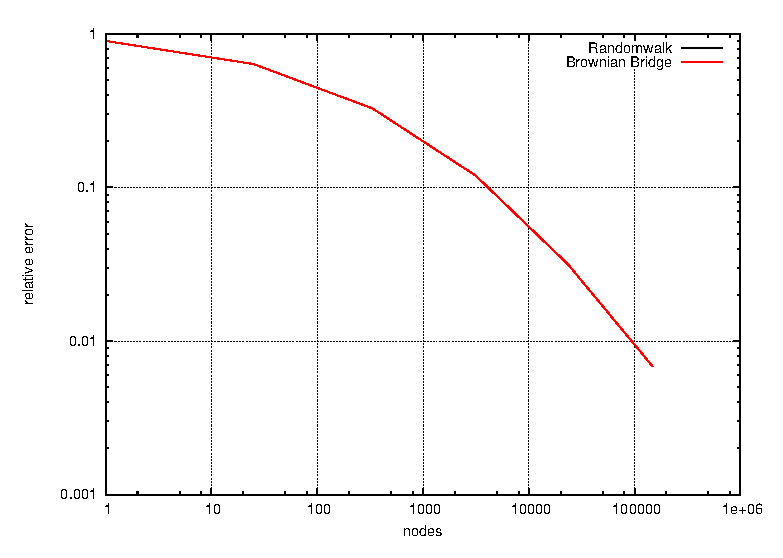
\includegraphics{task16_trapsparse}
\caption{Sparse grid trapezoidal rule}
\label{fig:Task16d}
\end{figure}

\begin{figure}[!ht]
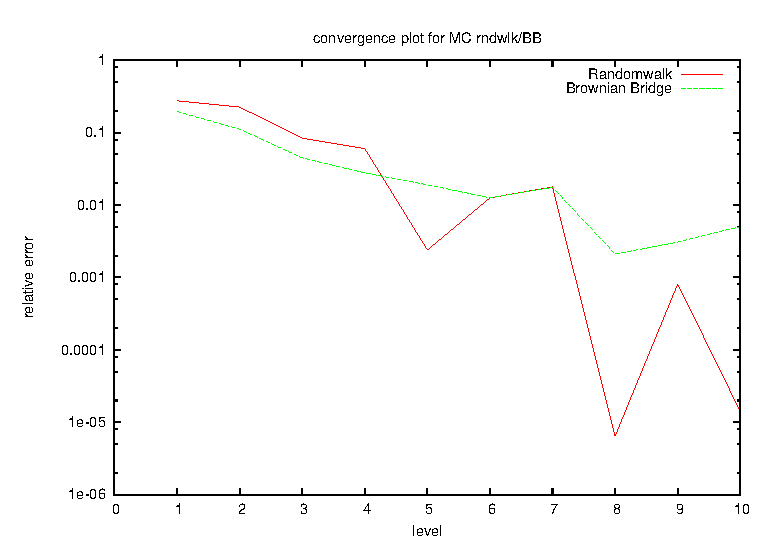
\includegraphics{task16_mc}
\caption{Monte-Carlo}
\label{fig:Task16e}
\end{figure}

\begin{figure}[!ht]
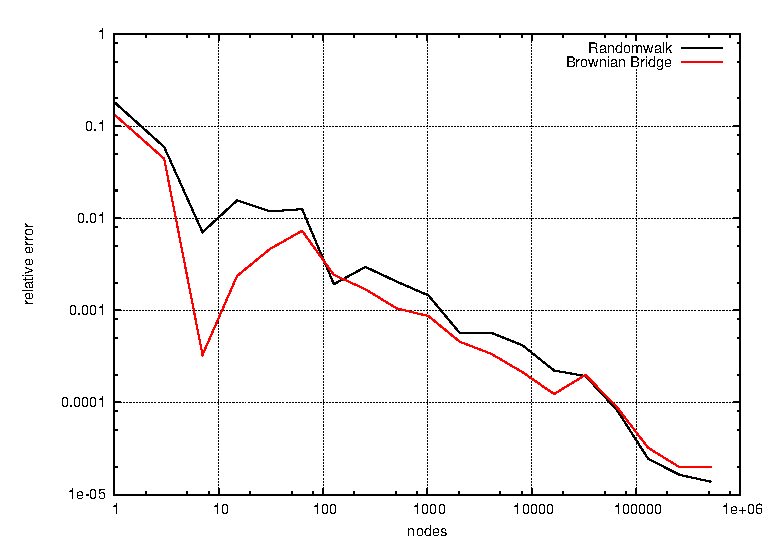
\includegraphics{task16_qmc}
\caption{Quasi-Monte-Carlo}
\label{fig:Task16f}
\end{figure}
\clearpage


\section*{Task 17}
Same as Task 16, but $K=10,M=64$.
\begin{figure}[!ht]
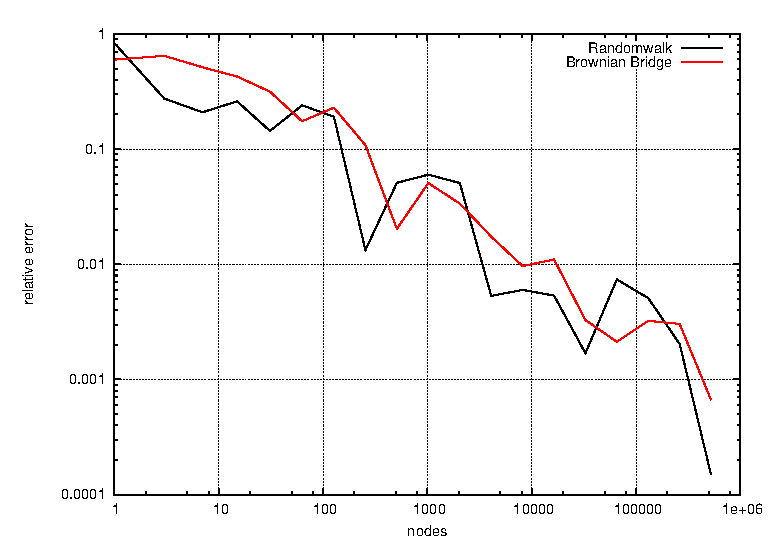
\includegraphics{task17_mc}
\caption{Monte-Carlo}
\label{fig:Task17a}
\end{figure}

\begin{figure}[!ht]
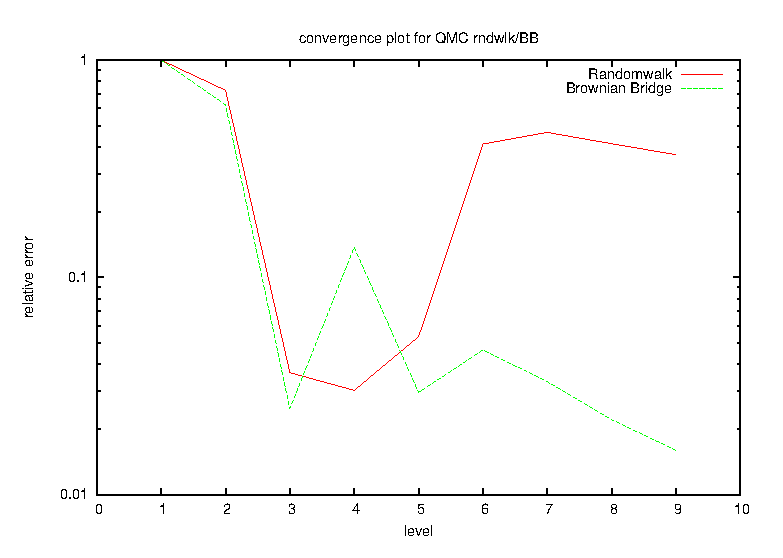
\includegraphics{task17_qmc}
\caption{Quasi-Monte-Carlo}
\label{fig:Task17b}
\end{figure}
\clearpage



\section*{Task 18} It is almost always better to not use (Q)MC, since the other
quadrature rules converge faster (even using full grids). Clenshaw-Curtis
converges slightly faster than the Trapezoidal rule. In almost all cases sparse
grids are preferrable Since they only give us a slightly worse convergences, but
way less points of evaluation (see Task 12). But if everything else fails, (Q)MC
works (but might converge slowly).
\end{document}
